\documentclass[12pt]{article}
\usepackage[utf8]{inputenc}
\usepackage{amsmath, amsthm, amssymb}
\usepackage{hyperref}
\usepackage{geometry}
\usepackage{listings}
\usepackage{xcolor}
\usepackage{graphicx}
\geometry{margin=1in}
\hypersetup{colorlinks=true,linkcolor=blue,citecolor=blue,urlcolor=blue}

\lstset{basicstyle=\ttfamily\small,breaklines=true,frame=single,backgroundcolor=\color{gray!6},columns=fullflexible}

\title{True String via Unordered-Pair Collision-Zero Encoding: Rigorous Structure and Empirical Profiles}
\author{Gabriel Neal Christensen \and Noah James Christensen}
\date{\today}

\theoremstyle{definition}
\newtheorem{definition}{Definition}[section]
\theoremstyle{plain}
\newtheorem{lemma}[definition]{Lemma}
\newtheorem{theorem}[definition]{Theorem}
\newtheorem{corollary}[definition]{Corollary}
\theoremstyle{remark}
\newtheorem{remark}[definition]{Remark}

\begin{document}
\maketitle

\begin{abstract}
We study the quadratic form \(g(m,n)=4+3m+3n+2mn\) and define a collision-zero encoding over unordered pairs \(\{m,n\}\). We prove exact structural results via the identity \(2g(m,n)+1=(2m+3)(2n+3)\): coverage of all odd composites and closed-form multiplicity counts. We separate rigorous theorems from empirical observations (residue profiles, density glimpses). No claim regarding the Riemann Hypothesis is made beyond empirical discussion.
\end{abstract}

\tableofcontents
\newpage

\section{Definitions}
\begin{definition}[Quadratic form]
\(g:\mathbb{N}_0\times\mathbb{N}_0\to\mathbb{N}\), \(g(m,n)=4+3m+3n+2mn\).
\end{definition}

\begin{definition}[Unordered-pair image and collision-zero encoding]
Let \(\mathcal{P}=\{\{m,n\}:m,n\in\mathbb{N}_0,\ m\le n\}\). For \(k\in\mathbb{N}\), let \(r_{un}(k)=\#\{\{m,n\}\in\mathcal{P}:g(m,n)=k\}\). Define
\[
T[k]=\begin{cases}k,& r_{un}(k)=1,\\0,& r_{un}(k)\ge 2,\\0,&k\notin g(\mathcal{P}).\end{cases}
\]
\end{definition}

\subsection*{Notation}
\(\mathbb{N}_0=\{0,1,2,\dots\}\). For odd \(c\ge 1\), \(d_{\mathrm{odd}}(c)\) is the number of odd divisors of \(c\). We write \(c\) square/non-square to indicate whether \(c\) is a perfect square.

\begin{center}
\begin{tabular}{l l}
Symbol & Meaning \\
\hline
\(\mathbb{N}_0\) & Nonnegative integers \\
\(g(m,n)\) & \(4+3m+3n+2mn\) \\
\(T[k]\) & Collision-zero encoding at value \(k\) (0 if repeated) \\
\(d_{\mathrm{odd}}(c)\) & Number of odd divisors of odd \(c\) \\
\end{tabular}
\end{center}

\section{Rigorous structure}
\begin{lemma}[Factorization identity]\label{lem:fact}
For all \(m,n\in\mathbb{N}_0\), \(2g(m,n)+1=(2m+3)(2n+3)\).
\end{lemma}
\begin{proof}
Let \(a=m+1\), \(b=n+1\). Then \(g=2ab+a+b\), so \(2g+1=(2a+1)(2b+1)=(2m+3)(2n+3)\).
\end{proof}

\begin{theorem}[Coverage of odd composites]\label{thm:coverage}
For every odd composite \(c\ge 9\), there exist \(m,n\in\mathbb{N}_0\) with \(2g(m,n)+1=c\).
\end{theorem}
\begin{proof}
Write \(c=uv\) with odd \(u,v\ge 3\). Set \(m=(u-3)/2\), \(n=(v-3)/2\); by Lemma~\ref{lem:fact}, \(2g(m,n)+1=(2m+3)(2n+3)=uv=c\).
\end{proof}

\begin{corollary}[Unordered multiplicity for \(2g+1\)]\label{cor:mult}
Let \(c\ge 9\) be odd composite. The number of unordered preimages \(\{m,n\}\) with \(2g(m,n)+1=c\) equals
\[
U(c)=\begin{cases}\dfrac{d_{\mathrm{odd}}(c)-2}{2},& c\text{ non-square},\\[6pt]
\dfrac{d_{\mathrm{odd}}(c)-2+1}{2},& c\text{ square},\end{cases}
\]
that is, \(U(c)=\lceil(d_{\mathrm{odd}}(c)-2)/2\rceil\).
\end{corollary}
\begin{proof}
Odd divisors of \(c\) other than \(1,c\) pair as \((u,c/u)\). For non-squares, all pairs have \(u\ne c/u\), giving \((d_{\mathrm{odd}}(c)-2)/2\) unordered pairs. For squares, one divisor equals \(\sqrt{c}\) and contributes a self-pair, adding \(1\) to \((d_{\mathrm{odd}}(c)-3)/2\), hence \((d_{\mathrm{odd}}(c)-2+1)/2\).
\end{proof}

\begin{remark}[On prime outputs of \(g\)]\label{rem:prime}
The identity of Lemma~\ref{lem:fact} concerns \(2g+1\), not \(g\) itself. Whether a prime value \(p=g(m,n)\) admits multiple unordered representations is a Diophantine question unrelated to factorization of \(2g+1\). We therefore avoid claiming uniqueness for prime outputs and treat any such phenomenon as empirical.
\end{remark}

\section{Empirical profiles}
Residue distributions and small-prime divisibility among distinct outputs \(g(\mathcal{P}\cap[0,M]^2)\) can be generated with the provided scripts. Figures (if generated) are placed under \texttt{fig/}.

\subsection*{Figures}
\begin{figure}[h]
\centering
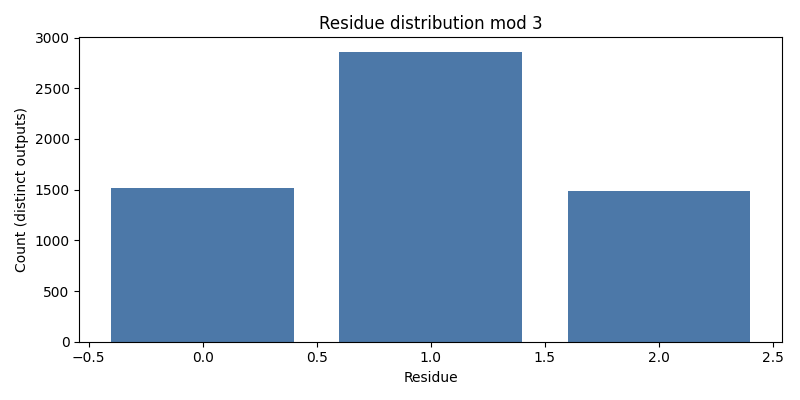
\includegraphics[width=0.7\linewidth]{../fig/residues_mod_3.png}
\caption{Residue distribution modulo 3 among distinct outputs for \(m,n\le 120\).}
\label{fig:u-mod3}
\end{figure}

\begin{figure}[h]
\centering
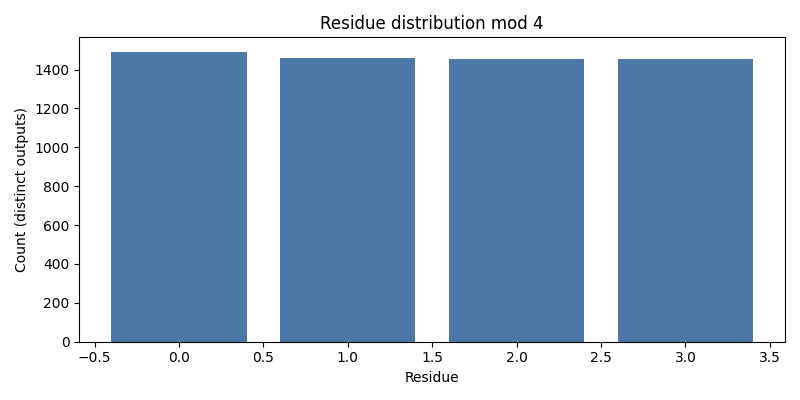
\includegraphics[width=0.7\linewidth]{../fig/residues_mod_4.png}
\caption{Residue distribution modulo 4 among distinct outputs for \(m,n\le 120\).}
\label{fig:u-mod4}
\end{figure}

\begin{figure}[h]
\centering
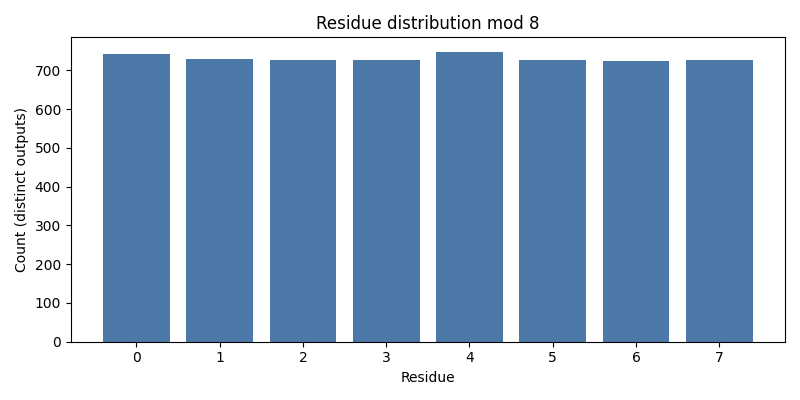
\includegraphics[width=0.7\linewidth]{../fig/residues_mod_8.png}
\caption{Residue distribution modulo 8 among distinct outputs for \(m,n\le 120\).}
\label{fig:u-mod8}
\end{figure}

\section{Reproducibility}
\begin{lstlisting}[language=bash]
# Build PDFs
make paper

# Profiles and plots
make profiles
make plots

# Verify coverage (ordered) and unordered multiplicity sampling
python3 python/test_parametric_odd_composites.py 200000
python3 python/verify_unordered_multiplicity.py 100000
\end{lstlisting}

\end{document}